%% Crisis Management Playbook Report
%% Enterprise-Level LaTeX Document Template
%% Compile with: pdflatex or xelatex (run twice for TOC)

\documentclass[11pt,a4paper]{article}

% ============================================
% PACKAGES
% ============================================
\usepackage[utf8]{inputenc}
\usepackage[T1]{fontenc}
\usepackage{geometry}
\usepackage{graphicx}
\usepackage{xcolor}
\usepackage{titlesec}
\usepackage{fancyhdr}
\usepackage{booktabs}
\usepackage{longtable}
\usepackage{array}
\usepackage{tabularx}
\usepackage{multirow}
\usepackage{enumitem}
\usepackage{tikz}
\usepackage{calc}
\usepackage{lastpage}
\usepackage{hyperref}
\usepackage{tcolorbox}
\usepackage{colortbl}
\usepackage{ragged2e}
\usepackage{amssymb}

% TikZ Libraries for Flow Diagrams
\usetikzlibrary{shapes.geometric, arrows.meta, positioning, calc, backgrounds, fit, decorations.pathreplacing}

% ============================================
% PAGE GEOMETRY
% ============================================
\geometry{
    top=2.5cm,
    bottom=2.5cm,
    left=2cm,
    right=2cm,
    headheight=1.5cm,
    footskip=1.5cm
}

% ============================================
% COLOR DEFINITIONS (Enterprise Palette)
% ============================================
\definecolor{primaryDark}{RGB}{31, 41, 55}      % gray-800
\definecolor{primaryLight}{RGB}{249, 250, 251}  % gray-50
\definecolor{borderGray}{RGB}{229, 231, 235}    % gray-200
\definecolor{textPrimary}{RGB}{17, 24, 39}      % gray-900
\definecolor{textSecondary}{RGB}{107, 114, 128} % gray-500
\definecolor{criticalRed}{RGB}{185, 28, 28}     % red-700
\definecolor{warningAmber}{RGB}{180, 83, 9}     % amber-700
\definecolor{successGreen}{RGB}{21, 128, 61}    % green-700 (only for success)

% ============================================
% HEADER/FOOTER CONFIGURATION
% ============================================
\pagestyle{fancy}
\fancyhf{}
\fancyhead[L]{\small\textcolor{textSecondary}{CRISIS MANAGEMENT REPORT}}
\fancyhead[R]{\small\textcolor{criticalRed}{\textbf{CONFIDENTIAL}}}
\fancyfoot[L]{\small\textcolor{textSecondary}{Document ID: CMP-2024-001}}
\fancyfoot[C]{\small\textcolor{textSecondary}{Page \thepage\ of \pageref{LastPage}}}
\fancyfoot[R]{\small\textcolor{textSecondary}{Generated: November 18, 2024}}
\renewcommand{\headrulewidth}{0.5pt}
\renewcommand{\footrulewidth}{0.5pt}

% ============================================
% SECTION FORMATTING
% ============================================
\titleformat{\section}
    {\normalfont\Large\bfseries\color{primaryDark}}
    {\thesection.}{0.5em}{}[\titlerule]
\titleformat{\subsection}
    {\normalfont\large\bfseries\color{primaryDark}}
    {\thesubsection}{0.5em}{}

% ============================================
% TCOLORBOX STYLES
% ============================================
\tcbuselibrary{skins, breakable}

\newtcolorbox{sectionbox}[1][]{
    enhanced,
    breakable,
    colback=white,
    colframe=borderGray,
    boxrule=0.5pt,
    arc=2pt,
    left=8pt,
    right=8pt,
    top=4pt,
    bottom=8pt,
    fonttitle=\small\bfseries,
    coltitle=white,
    attach boxed title to top left={xshift=0pt, yshift=-\tcboxedtitleheight},
    boxed title style={colback=primaryDark, colframe=primaryDark, arc=2pt, boxrule=0pt},
    title={\MakeUppercase{#1}}
}

\newtcolorbox{flowbox}{
    enhanced,
    colback=primaryLight,
    colframe=borderGray,
    boxrule=0.5pt,
    arc=3pt,
    left=10pt,
    right=10pt,
    top=10pt,
    bottom=10pt
}

% ============================================
% CUSTOM COMMANDS
% ============================================
\newcommand{\criticalbadge}[1]{%
    \tikz[baseline=(text.base)]{
        \node[fill=criticalRed, text=white, rounded corners=2pt, inner sep=2pt, font=\tiny\bfseries] (text) {#1};
    }%
}
\newcommand{\statusbadge}[2]{%
    \tikz[baseline=(text.base)]{
        \node[fill=#1, text=white, rounded corners=2pt, inner sep=2pt, font=\tiny\bfseries] (text) {#2};
    }%
}
\newcommand{\phasebadge}[1]{%
    \tikz[baseline=(text.base)]{
        \node[fill=primaryDark, text=white, rounded corners=2pt, inner sep=3pt, font=\scriptsize\bfseries] (text) {#1};
    }%
}


% ============================================
% DOCUMENT BEGINS
% ============================================
\begin{document}

% ============================================
% TITLE PAGE
% ============================================
\begin{titlepage}
\begin{tikzpicture}[remember picture, overlay]
    % Header bar
    \fill[primaryDark] (current page.north west) rectangle ([yshift=-3cm]current page.north east);
    \node[anchor=north west, text=white, font=\small] at ([xshift=2cm, yshift=-1cm]current page.north west) {ENTERPRISE CRISIS MANAGEMENT};
    \node[anchor=north east, text=white, font=\small\bfseries] at ([xshift=-2cm, yshift=-1cm]current page.north east) {CONFIDENTIAL};

    % Footer bar
    \fill[primaryDark] (current page.south west) rectangle ([yshift=1.5cm]current page.south east);
    \node[anchor=south, text=white, font=\small] at ([yshift=0.75cm]current page.south) {Acme Financial Services | Crisis Management Division};
\end{tikzpicture}

\vspace*{4cm}

\begin{center}
    {\Huge\bfseries\color{primaryDark} CRISIS MANAGEMENT}\\[0.3cm]
    {\Huge\bfseries\color{primaryDark} INCIDENT REPORT}\\[1.5cm]

    
\begin{tikzpicture}
        \node[fill=criticalRed, text=white, rounded corners=4pt, inner sep=10pt, font=\Large\bfseries] {SEVERITY: CRITICAL};
    \end{tikzpicture}

    \vspace{1.5cm}

    {\Large\bfseries Ransomware Attack Response}\\[0.2cm]
    {\Large Core Banking Systems}\\[1.5cm]

    \begin{tabular}{rl}
        \textcolor{textSecondary}{\small INCIDENT ID:} & \textbf{INC-2024-1115-001} \\[0.3cm]
        \textcolor{textSecondary}{\small DATE:} & \textbf{November 15-16, 2024} \\[0.3cm]
        \textcolor{textSecondary}{\small DURATION:} & \textbf{12 hours 43 minutes} \\[0.3cm]
        \textcolor{textSecondary}{\small STATUS:} & \statusbadge{primaryDark}{RESOLVED} \\
    \end{tabular}

    \vspace{2cm}

    \rule{0.6\textwidth}{0.5pt}\\[0.5cm]
    {\small Prepared by: Sarah Chen, Chief Information Security Officer}\\
    {\small\textcolor{textSecondary}{Document Version 1.0 | November 18, 2024}}
\end{center}
\end{titlepage}

% ============================================
% TABLE OF CONTENTS
% ============================================
\tableofcontents
\newpage

% ============================================
% INCIDENT FLOW VISUALIZATION
% ============================================
\section{Incident Flow Overview}

\begin{flowbox}
\begin{center}
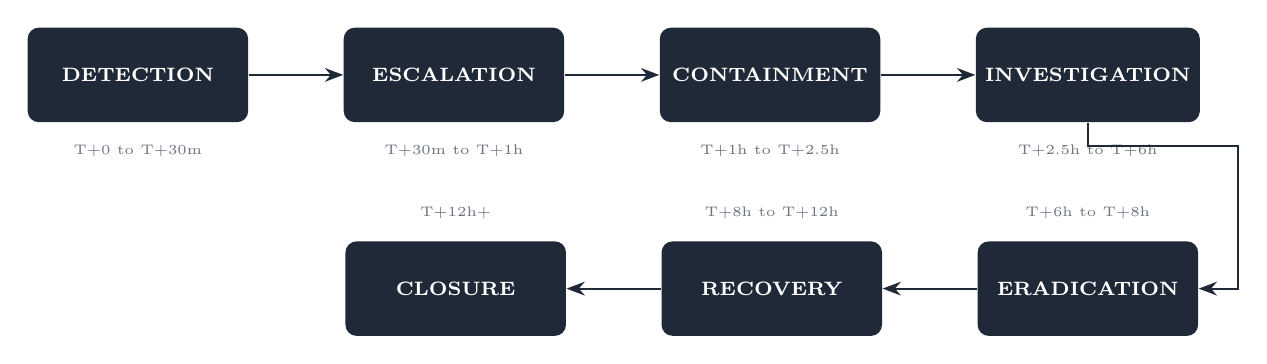
\begin{tikzpicture}[
    node distance=0.8cm and 1.2cm,
    % Node styles
    phase/.style={
        rectangle,
        rounded corners=4pt,
        minimum width=2.8cm,
        minimum height=1.2cm,
        text centered,
        font=\scriptsize\bfseries,
        text=white,
        fill=primaryDark
    },
    timenode/.style={
        rectangle,
        minimum width=2.8cm,
        minimum height=0.5cm,
        text centered,
        font=\tiny,
        text=textSecondary
    },
    arrow/.style={
        ->,
        >=Stealth,
        thick,
        color=primaryDark
    },
    timeline/.style={
        draw=borderGray,
        line width=2pt
    }
]

% Phase nodes - horizontal flow
\node[phase] (p1) {DETECTION};
\node[phase, right=of p1] (p2) {ESCALATION};
\node[phase, right=of p2] (p3) {CONTAINMENT};
\node[phase, right=of p3] (p4) {INVESTIGATION};

% Second row
\node[phase, below=1.5cm of p4] (p5) {ERADICATION};
\node[phase, left=of p5] (p6) {RECOVERY};
\node[phase, left=of p6] (p7) {CLOSURE};

% Time labels
\node[timenode, below=0.1cm of p1] {T+0 to T+30m};
\node[timenode, below=0.1cm of p2] {T+30m to T+1h};
\node[timenode, below=0.1cm of p3] {T+1h to T+2.5h};
\node[timenode, below=0.1cm of p4] {T+2.5h to T+6h};
\node[timenode, above=0.1cm of p5] {T+6h to T+8h};
\node[timenode, above=0.1cm of p6] {T+8h to T+12h};
\node[timenode, above=0.1cm of p7] {T+12h+};

% Arrows
\draw[arrow] (p1) -- (p2);
\draw[arrow] (p2) -- (p3);
\draw[arrow] (p3) -- (p4);
\draw[arrow] (p4) -- ([yshift=-0.3cm]p4.south) -| ([xshift=0.5cm]p5.east) -- (p5.east);
\draw[arrow] (p5) -- (p6);
\draw[arrow] (p6) -- (p7);

\end{tikzpicture}
\end{center}

\vspace{0.5cm}
\begin{center}
\small\textcolor{textSecondary}{Figure 1: High-Level Incident Response Phase Flow}
\end{center}
\end{flowbox}

\vspace{0.8cm}

% ============================================
% DETAILED INCIDENT TIMELINE
% ============================================
\begin{sectionbox}[Incident Timeline]
\begin{center}
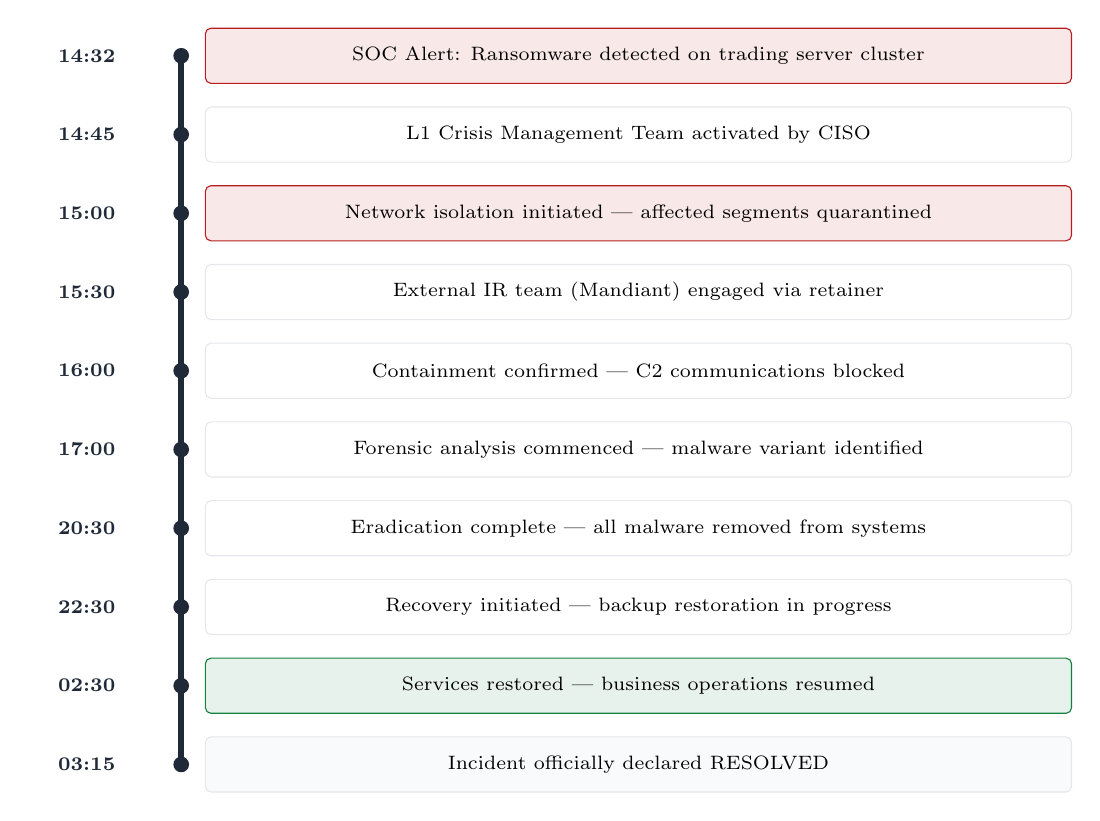
\begin{tikzpicture}[
    node distance=0.4cm,
    event/.style={
        rectangle,
        rounded corners=2pt,
        minimum width=11cm,
        minimum height=0.7cm,
        text centered,
        font=\scriptsize,
        draw=borderGray,
        fill=white,
        align=left
    },
    time/.style={
        rectangle,
        minimum width=1.5cm,
        text centered,
        font=\scriptsize\bfseries,
        text=primaryDark
    },
    critical/.style={
        event,
        fill=criticalRed!10,
        draw=criticalRed
    },
    milestone/.style={
        circle,
        fill=primaryDark,
        inner sep=2pt
    }
]

% Timeline line
\draw[line width=2pt, primaryDark] (0,0) -- (0,-9);

% Events
\node[time] at (-1.2, 0) {14:32};
\node[milestone] at (0, 0) {};
\node[critical, anchor=west] at (0.3, 0) {SOC Alert: Ransomware detected on trading server cluster};

\node[time] at (-1.2, -1) {14:45};
\node[milestone] at (0, -1) {};
\node[event, anchor=west] at (0.3, -1) {L1 Crisis Management Team activated by CISO};

\node[time] at (-1.2, -2) {15:00};
\node[milestone] at (0, -2) {};
\node[critical, anchor=west] at (0.3, -2) {Network isolation initiated --- affected segments quarantined};

\node[time] at (-1.2, -3) {15:30};
\node[milestone] at (0, -3) {};
\node[event, anchor=west] at (0.3, -3) {External IR team (Mandiant) engaged via retainer};

\node[time] at (-1.2, -4) {16:00};
\node[milestone] at (0, -4) {};
\node[event, anchor=west] at (0.3, -4) {Containment confirmed --- C2 communications blocked};

\node[time] at (-1.2, -5) {17:00};
\node[milestone] at (0, -5) {};
\node[event, anchor=west] at (0.3, -5) {Forensic analysis commenced --- malware variant identified};

\node[time] at (-1.2, -6) {20:30};
\node[milestone] at (0, -6) {};
\node[event, anchor=west] at (0.3, -6) {Eradication complete --- all malware removed from systems};

\node[time] at (-1.2, -7) {22:30};
\node[milestone] at (0, -7) {};
\node[event, anchor=west] at (0.3, -7) {Recovery initiated --- backup restoration in progress};

\node[time] at (-1.2, -8) {02:30};
\node[milestone] at (0, -8) {};
\node[event, anchor=west, fill=successGreen!10, draw=successGreen] at (0.3, -8) {Services restored --- business operations resumed};

\node[time] at (-1.2, -9) {03:15};
\node[milestone] at (0, -9) {};
\node[event, anchor=west, fill=primaryLight] at (0.3, -9) {Incident officially declared RESOLVED};

\end{tikzpicture}
\end{center}

\vspace{0.3cm}
\begin{center}
\small\textcolor{textSecondary}{Figure 2: Incident Timeline (All times in UTC)}
\end{center}
\end{sectionbox}

\newpage

% ============================================
% ESCALATION FLOW DIAGRAM
% ============================================
\begin{sectionbox}[Team Escalation Flow]
\begin{center}
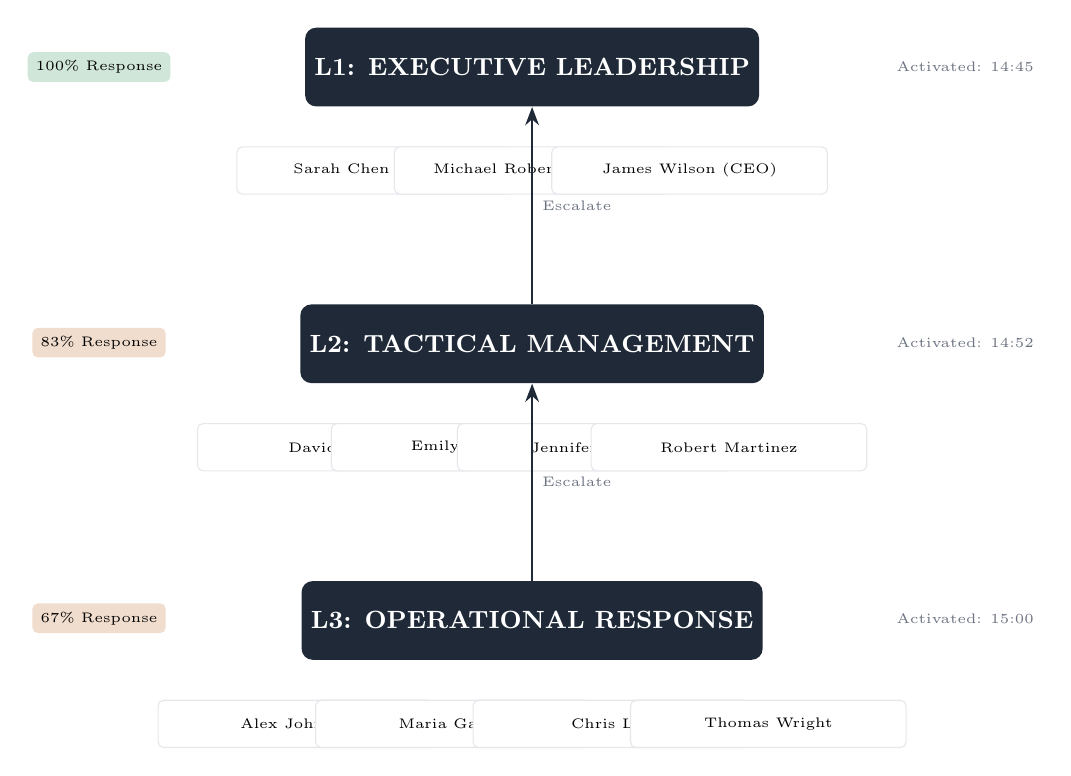
\begin{tikzpicture}[
    node distance=1cm and 2cm,
    level/.style={
        rectangle,
        rounded corners=4pt,
        minimum width=4cm,
        minimum height=1cm,
        text centered,
        font=\small\bfseries,
        text=white,
        fill=primaryDark
    },
    person/.style={
        rectangle,
        rounded corners=2pt,
        minimum width=3.5cm,
        minimum height=0.6cm,
        text centered,
        font=\tiny,
        draw=borderGray,
        fill=white
    },
    arrow/.style={
        ->,
        >=Stealth,
        thick,
        color=primaryDark
    },
    dashedarrow/.style={
        ->,
        >=Stealth,
        dashed,
        color=textSecondary
    }
]

% L1 - Strategic
\node[level] (l1) {L1: EXECUTIVE LEADERSHIP};
\node[person, below=0.5cm of l1, xshift=-2cm] (l1a) {Sarah Chen (CISO)};
\node[person, below=0.5cm of l1] (l1b) {Michael Roberts (CTO)};
\node[person, below=0.5cm of l1, xshift=2cm] (l1c) {James Wilson (CEO)};

% L2 - Tactical
\node[level, below=2.5cm of l1] (l2) {L2: TACTICAL MANAGEMENT};
\node[person, below=0.5cm of l2, xshift=-2.5cm] (l2a) {David Park};
\node[person, below=0.5cm of l2, xshift=-0.8cm] (l2b) {Emily Watson};
\node[person, below=0.5cm of l2, xshift=0.8cm] (l2c) {Jennifer Adams};
\node[person, below=0.5cm of l2, xshift=2.5cm] (l2d) {Robert Martinez};

% L3 - Operational
\node[level, below=2.5cm of l2] (l3) {L3: OPERATIONAL RESPONSE};
\node[person, below=0.5cm of l3, xshift=-3cm] (l3a) {Alex Johnson};
\node[person, below=0.5cm of l3, xshift=-1cm] (l3b) {Maria Garcia};
\node[person, below=0.5cm of l3, xshift=1cm] (l3c) {Chris Lee};
\node[person, below=0.5cm of l3, xshift=3cm] (l3d) {Thomas Wright};

% Escalation arrows
\draw[arrow] (l3) -- node[right, font=\tiny, text=textSecondary] {Escalate} (l2);
\draw[arrow] (l2) -- node[right, font=\tiny, text=textSecondary] {Escalate} (l1);

% Time annotations
\node[font=\tiny, text=textSecondary] at (5.5, 0) {Activated: 14:45};
\node[font=\tiny, text=textSecondary] at (5.5, -3.5) {Activated: 14:52};
\node[font=\tiny, text=textSecondary] at (5.5, -7) {Activated: 15:00};

% Response rate boxes
\node[fill=successGreen!20, rounded corners=2pt, font=\tiny, inner sep=3pt] at (-5.5, 0) {100\% Response};
\node[fill=warningAmber!20, rounded corners=2pt, font=\tiny, inner sep=3pt] at (-5.5, -3.5) {83\% Response};
\node[fill=warningAmber!20, rounded corners=2pt, font=\tiny, inner sep=3pt] at (-5.5, -7) {67\% Response};

\end{tikzpicture}
\end{center}

\vspace{0.3cm}
\begin{center}
\small\textcolor{textSecondary}{Figure 3: Crisis Management Team Escalation Hierarchy}
\end{center}
\end{sectionbox}

\newpage

% ============================================
% ATTACK CHAIN VISUALIZATION
% ============================================
\begin{sectionbox}[Attack Chain Analysis]
\begin{center}
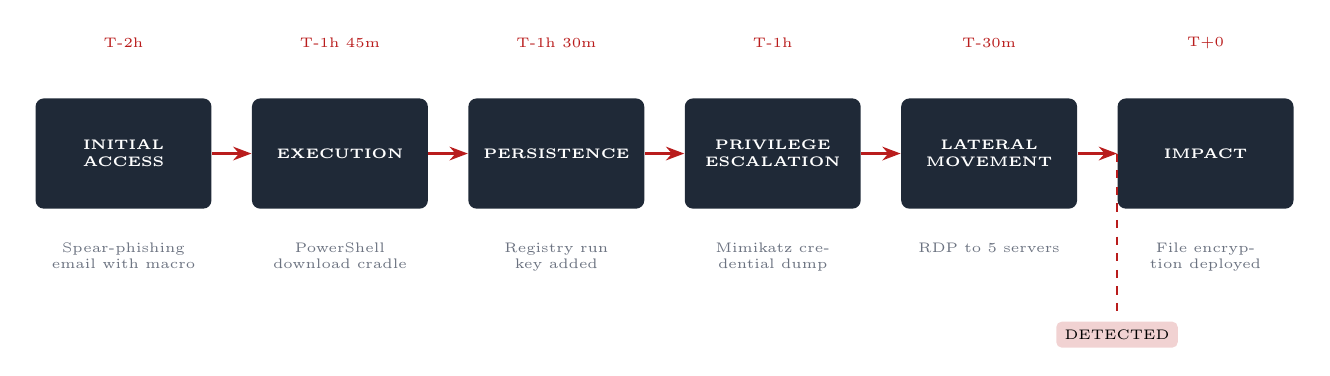
\begin{tikzpicture}[
    node distance=0.3cm and 0.5cm,
    attackstep/.style={
        rectangle,
        rounded corners=3pt,
        minimum width=2.2cm,
        minimum height=1.4cm,
        text centered,
        font=\tiny\bfseries,
        text=white,
        fill=primaryDark,
        text width=2cm
    },
    detail/.style={
        rectangle,
        rounded corners=2pt,
        minimum width=2.2cm,
        text centered,
        font=\tiny,
        text=textSecondary,
        text width=2.2cm
    },
    arrow/.style={
        ->,
        >=Stealth,
        thick,
        color=criticalRed
    }
]

% Attack chain nodes
\node[attackstep] (a1) {INITIAL\\ACCESS};
\node[attackstep, right=of a1] (a2) {EXECUTION};
\node[attackstep, right=of a2] (a3) {PERSISTENCE};
\node[attackstep, right=of a3] (a4) {PRIVILEGE\\ESCALATION};
\node[attackstep, right=of a4] (a5) {LATERAL\\MOVEMENT};
\node[attackstep, right=of a5] (a6) {IMPACT};

% Details below
\node[detail, below=0.3cm of a1] {Spear-phishing email with macro};
\node[detail, below=0.3cm of a2] {PowerShell download cradle};
\node[detail, below=0.3cm of a3] {Registry run key added};
\node[detail, below=0.3cm of a4] {Mimikatz credential dump};
\node[detail, below=0.3cm of a5] {RDP to 5 servers};
\node[detail, below=0.3cm of a6] {File encryption deployed};

% Arrows
\draw[arrow] (a1) -- (a2);
\draw[arrow] (a2) -- (a3);
\draw[arrow] (a3) -- (a4);
\draw[arrow] (a4) -- (a5);
\draw[arrow] (a5) -- (a6);

% Time indicators
\node[font=\tiny, text=criticalRed] at ([yshift=0.7cm]a1.north) {T-2h};
\node[font=\tiny, text=criticalRed] at ([yshift=0.7cm]a2.north) {T-1h 45m};
\node[font=\tiny, text=criticalRed] at ([yshift=0.7cm]a3.north) {T-1h 30m};
\node[font=\tiny, text=criticalRed] at ([yshift=0.7cm]a4.north) {T-1h};
\node[font=\tiny, text=criticalRed] at ([yshift=0.7cm]a5.north) {T-30m};
\node[font=\tiny, text=criticalRed] at ([yshift=0.7cm]a6.north) {T+0};

% Detection point
\draw[dashed, criticalRed, thick] ([xshift=0.5cm]a5.east) -- ([xshift=0.5cm, yshift=-2cm]a5.east);
\node[fill=criticalRed!20, rounded corners=2pt, font=\tiny, inner sep=3pt] at ([xshift=0.5cm, yshift=-2.3cm]a5.east) {DETECTED};

\end{tikzpicture}
\end{center}

\vspace{0.3cm}
\begin{center}
\small\textcolor{textSecondary}{Figure 4: MITRE ATT\&CK Chain --- Ransomware Kill Chain}
\end{center}
\end{sectionbox}

\vspace{0.8cm}

% ============================================
% RESPONSE ACTIONS FLOW
% ============================================
\begin{sectionbox}[Response Actions by Phase]
\begin{center}
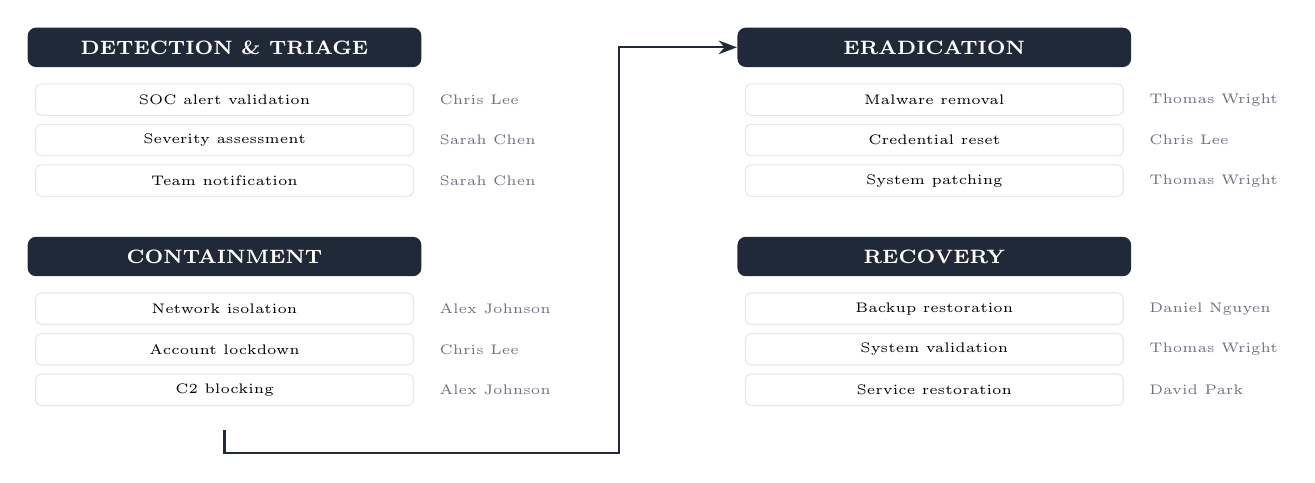
\begin{tikzpicture}[
    node distance=0.2cm,
    phasebox/.style={
        rectangle,
        rounded corners=3pt,
        minimum width=5cm,
        minimum height=0.5cm,
        text centered,
        font=\scriptsize\bfseries,
        text=white,
        fill=primaryDark
    },
    actionbox/.style={
        rectangle,
        rounded corners=2pt,
        minimum width=4.8cm,
        minimum height=0.4cm,
        text centered,
        font=\tiny,
        draw=borderGray,
        fill=white
    },
    responder/.style={
        font=\tiny,
        text=textSecondary
    }
]

% Left column - Detection & Containment
\node[phasebox] (p1) {DETECTION \& TRIAGE};
\node[actionbox, below=0.2cm of p1] (a1) {SOC alert validation};
\node[responder, right=0.2cm of a1] {Chris Lee};
\node[actionbox, below=0.1cm of a1] (a2) {Severity assessment};
\node[responder, right=0.2cm of a2] {Sarah Chen};
\node[actionbox, below=0.1cm of a2] (a3) {Team notification};
\node[responder, right=0.2cm of a3] {Sarah Chen};

\node[phasebox, below=0.5cm of a3] (p2) {CONTAINMENT};
\node[actionbox, below=0.2cm of p2] (a4) {Network isolation};
\node[responder, right=0.2cm of a4] {Alex Johnson};
\node[actionbox, below=0.1cm of a4] (a5) {Account lockdown};
\node[responder, right=0.2cm of a5] {Chris Lee};
\node[actionbox, below=0.1cm of a5] (a6) {C2 blocking};
\node[responder, right=0.2cm of a6] {Alex Johnson};

% Right column - Eradication & Recovery
\node[phasebox, right=4cm of p1] (p3) {ERADICATION};
\node[actionbox, below=0.2cm of p3] (b1) {Malware removal};
\node[responder, right=0.2cm of b1] {Thomas Wright};
\node[actionbox, below=0.1cm of b1] (b2) {Credential reset};
\node[responder, right=0.2cm of b2] {Chris Lee};
\node[actionbox, below=0.1cm of b2] (b3) {System patching};
\node[responder, right=0.2cm of b3] {Thomas Wright};

\node[phasebox, below=0.5cm of b3] (p4) {RECOVERY};
\node[actionbox, below=0.2cm of p4] (b4) {Backup restoration};
\node[responder, right=0.2cm of b4] {Daniel Nguyen};
\node[actionbox, below=0.1cm of b4] (b5) {System validation};
\node[responder, right=0.2cm of b5] {Thomas Wright};
\node[actionbox, below=0.1cm of b5] (b6) {Service restoration};
\node[responder, right=0.2cm of b6] {David Park};

% Connecting arrows
\draw[->, >=Stealth, thick, primaryDark] ([yshift=-0.3cm]a6.south) -- ([yshift=-0.6cm]a6.south) -| ([xshift=-1.5cm]p3.west) -- (p3.west);

\end{tikzpicture}
\end{center}

\vspace{0.3cm}
\begin{center}
\small\textcolor{textSecondary}{Figure 5: Response Actions with Assigned Responders}
\end{center}
\end{sectionbox}

\newpage

% ============================================
% IMPACT RADIUS DIAGRAM
% ============================================
\begin{sectionbox}[Impact Radius \& Affected Systems]
\begin{center}
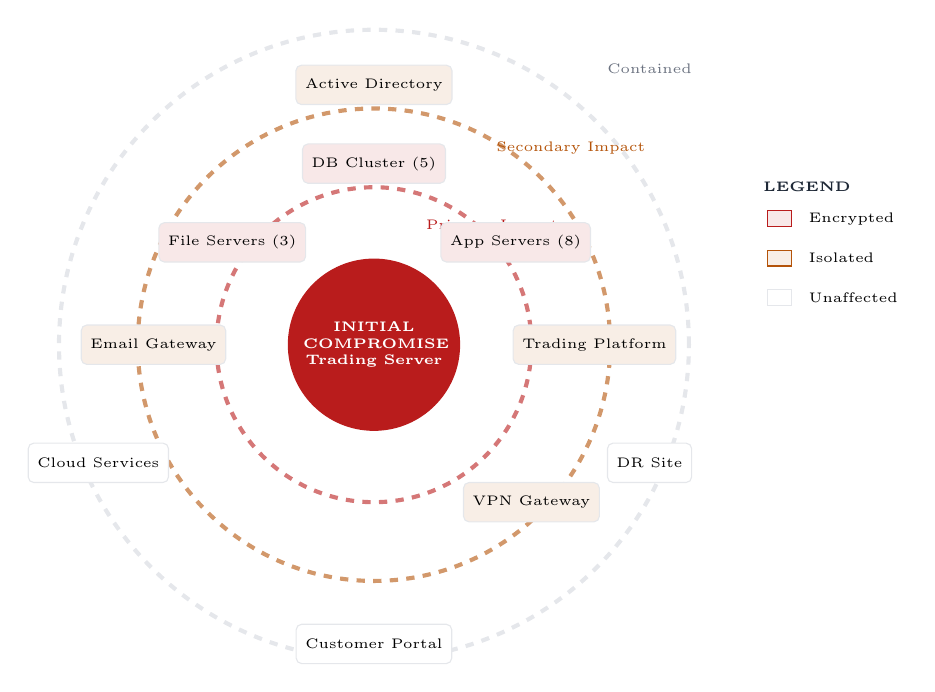
\begin{tikzpicture}[
    node distance=0.5cm,
    core/.style={
        circle,
        minimum size=2cm,
        text centered,
        font=\tiny\bfseries,
        text=white,
        fill=criticalRed,
        text width=1.8cm
    },
    ring1/.style={
        circle,
        minimum size=4cm,
        draw=criticalRed!60,
        line width=1.5pt,
        dashed
    },
    ring2/.style={
        circle,
        minimum size=6cm,
        draw=warningAmber!60,
        line width=1.5pt,
        dashed
    },
    ring3/.style={
        circle,
        minimum size=8cm,
        draw=borderGray,
        line width=1.5pt,
        dashed
    },
    sysbox/.style={
        rectangle,
        rounded corners=2pt,
        minimum height=0.5cm,
        text centered,
        font=\tiny,
        fill=white,
        draw=borderGray
    }
]

% Concentric rings
\node[ring3] at (0,0) {};
\node[ring2] at (0,0) {};
\node[ring1] at (0,0) {};
\node[core] (center) {INITIAL\\COMPROMISE\\Trading Server};

% Ring labels
\node[font=\tiny, text=criticalRed] at (1.5, 1.5) {Primary Impact};
\node[font=\tiny, text=warningAmber] at (2.5, 2.5) {Secondary Impact};
\node[font=\tiny, text=textSecondary] at (3.5, 3.5) {Contained};

% Affected systems around the rings
\node[sysbox, fill=criticalRed!10] at (0, 2.3) {DB Cluster (5)};
\node[sysbox, fill=criticalRed!10] at (1.8, 1.3) {App Servers (8)};
\node[sysbox, fill=criticalRed!10] at (-1.8, 1.3) {File Servers (3)};

\node[sysbox, fill=warningAmber!10] at (0, 3.3) {Active Directory};
\node[sysbox, fill=warningAmber!10] at (2.8, 0) {Trading Platform};
\node[sysbox, fill=warningAmber!10] at (-2.8, 0) {Email Gateway};
\node[sysbox, fill=warningAmber!10] at (2, -2) {VPN Gateway};

\node[sysbox] at (0, -3.8) {Customer Portal};
\node[sysbox] at (3.5, -1.5) {DR Site};
\node[sysbox] at (-3.5, -1.5) {Cloud Services};

% Legend
\node[font=\tiny\bfseries, text=primaryDark] at (5.5, 2) {LEGEND};
\draw[fill=criticalRed!10, draw=criticalRed] (5, 1.5) rectangle (5.3, 1.7);
\node[font=\tiny, anchor=west] at (5.4, 1.6) {Encrypted};
\draw[fill=warningAmber!10, draw=warningAmber] (5, 1) rectangle (5.3, 1.2);
\node[font=\tiny, anchor=west] at (5.4, 1.1) {Isolated};
\draw[fill=white, draw=borderGray] (5, 0.5) rectangle (5.3, 0.7);
\node[font=\tiny, anchor=west] at (5.4, 0.6) {Unaffected};

\end{tikzpicture}
\end{center}

\vspace{0.3cm}
\begin{center}
\small\textcolor{textSecondary}{Figure 6: Impact Radius --- Systems Affected by Proximity to Initial Compromise}
\end{center}
\end{sectionbox}

\vspace{0.8cm}

% ============================================
% COMMUNICATIONS FLOW DIAGRAM
% ============================================
\begin{sectionbox}[Crisis Communications Flow]
\begin{center}
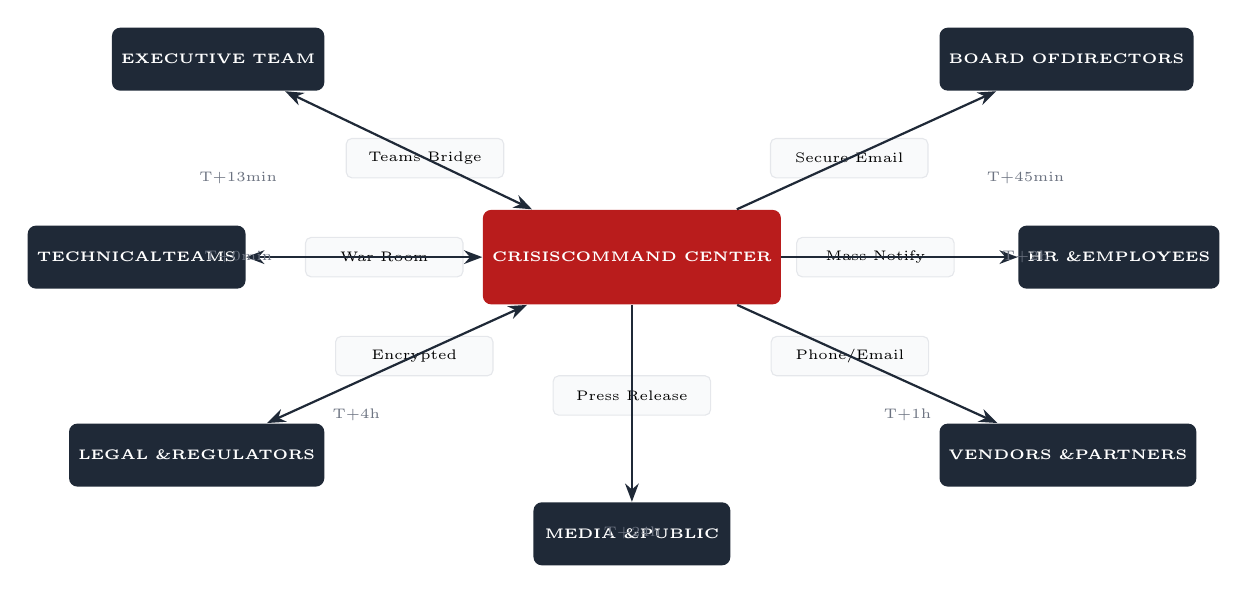
\begin{tikzpicture}[
    node distance=0.6cm and 1.5cm,
    stakeholder/.style={
        rectangle,
        rounded corners=3pt,
        minimum width=2.5cm,
        minimum height=0.8cm,
        text centered,
        font=\tiny\bfseries,
        text=white,
        fill=primaryDark
    },
    channel/.style={
        rectangle,
        rounded corners=2pt,
        minimum width=2cm,
        minimum height=0.5cm,
        text centered,
        font=\tiny,
        draw=borderGray,
        fill=primaryLight
    },
    arrow/.style={
        ->,
        >=Stealth,
        thick,
        color=primaryDark
    },
    bidir/.style={
        <->,
        >=Stealth,
        thick,
        color=primaryDark
    }
]

% Central Command
\node[stakeholder, minimum width=3.5cm, minimum height=1.2cm, fill=criticalRed] (cmd) {CRISIS\\COMMAND CENTER};

% Internal stakeholders
\node[stakeholder, above left=1.5cm and 2cm of cmd] (exec) {EXECUTIVE TEAM};
\node[stakeholder, above right=1.5cm and 2cm of cmd] (board) {BOARD OF\\DIRECTORS};
\node[stakeholder, left=3cm of cmd] (tech) {TECHNICAL\\TEAMS};
\node[stakeholder, right=3cm of cmd] (hr) {HR \&\\EMPLOYEES};

% External stakeholders
\node[stakeholder, below left=1.5cm and 2cm of cmd] (legal) {LEGAL \&\\REGULATORS};
\node[stakeholder, below right=1.5cm and 2cm of cmd] (vendor) {VENDORS \&\\PARTNERS};
\node[stakeholder, below=2.5cm of cmd] (media) {MEDIA \&\\PUBLIC};

% Channels
\node[channel] at ($(cmd)!0.5!(exec)$) {Teams Bridge};
\node[channel] at ($(cmd)!0.5!(board)$) {Secure Email};
\node[channel] at ($(cmd)!0.5!(tech)$) {War Room};
\node[channel] at ($(cmd)!0.5!(hr)$) {Mass Notify};
\node[channel] at ($(cmd)!0.5!(legal)$) {Encrypted};
\node[channel] at ($(cmd)!0.5!(vendor)$) {Phone/Email};
\node[channel] at ($(cmd)!0.5!(media)$) {Press Release};

% Arrows
\draw[bidir] (cmd) -- (exec);
\draw[arrow] (cmd) -- (board);
\draw[bidir] (cmd) -- (tech);
\draw[arrow] (cmd) -- (hr);
\draw[bidir] (cmd) -- (legal);
\draw[arrow] (cmd) -- (vendor);
\draw[arrow] (cmd) -- (media);

% Timing annotations
\node[font=\tiny, text=textSecondary] at (-5, 1) {T+13min};
\node[font=\tiny, text=textSecondary] at (5, 1) {T+45min};
\node[font=\tiny, text=textSecondary] at (-5, 0) {T+0min};
\node[font=\tiny, text=textSecondary] at (5, 0) {T+2h};
\node[font=\tiny, text=textSecondary] at (-3.5, -2) {T+4h};
\node[font=\tiny, text=textSecondary] at (3.5, -2) {T+1h};
\node[font=\tiny, text=textSecondary] at (0, -3.5) {T+24h};

\end{tikzpicture}
\end{center}

\vspace{0.3cm}
\begin{center}
\small\textcolor{textSecondary}{Figure 7: Crisis Communications Flow with Stakeholder Notification Timing}
\end{center}
\end{sectionbox}

\newpage

% ============================================
% SECTION 2: INCIDENT CLASSIFICATION
% ============================================
\section{Incident Classification}

\begin{sectionbox}[Classification Details]
\begin{tabularx}{\textwidth}{@{}lXlX@{}}
    \toprule
    \textcolor{textSecondary}{\scriptsize PLAYBOOK NAME} & Ransomware Attack Response & \textcolor{textSecondary}{\scriptsize CATEGORY} & Cyber Security Incident \\
    \midrule
    \textcolor{textSecondary}{\scriptsize INCIDENT TYPE} & Ransomware/Malware & \textcolor{textSecondary}{\scriptsize SEVERITY} & \criticalbadge{CRITICAL} \\
    \midrule
    \textcolor{textSecondary}{\scriptsize INVOCATION} & YES --- Full Activation & \textcolor{textSecondary}{\scriptsize EST. DURATION} & 24--48 hours \\
    \midrule
    \textcolor{textSecondary}{\scriptsize OWNER} & Sarah Chen, CISO & \textcolor{textSecondary}{\scriptsize ACTUAL DURATION} & 12h 43min \\
    \bottomrule
\end{tabularx}

\vspace{0.5cm}
\textbf{Incident Description:}\\[0.2cm]
At 14:32 UTC on November 15, 2024, the Security Operations Center detected ransomware activity on the trading server cluster. The attack originated from a spear-phishing email targeting a senior trading analyst. The malware variant (LockBit 3.0) encrypted files on 23 systems before containment was achieved. No data exfiltration was confirmed. Full recovery was achieved within 12 hours 43 minutes.

\vspace{0.5cm}
\textbf{Impact Summary:}
\begin{itemize}[nosep,leftmargin=*]
    \item \textbf{Systems Affected:} 23 servers (trading, database, application tiers)
    \item \textbf{Users Impacted:} 2,847 internal users, 0 external customers
    \item \textbf{Data Loss:} None (restored from backups)
    \item \textbf{Financial Impact:} \$1.2M estimated (revenue loss + remediation)
\end{itemize}
\end{sectionbox}